\marginnote[0cm]{
\emph{\say{ Je me détourne avec effroi et horreur de cette plaie lamentable des fonctions continues qui n'ont point de dérivées. }} \\
\hspace*{\fill} Charles \textsc{Hermite} (1893) \\
\emph{\say{ C’est un cas où il est vraiment naturel de penser à ces fonctions continues sans dérivées que les mathématiciens ont imaginées, et que l’on regardait à tort comme de
simples curiosités mathématiques, puisque l’expérience peut les suggérer. }} \\
\hspace*{\fill} Jean \textsc{Perrin} \sidenote{Physicien, chimiste et homme politique français (1870 - 1942), prix Nobel de physique 1926.}, au sujet du mouvement brownien.
}

\cite{contre-exemples} p. 160 \\
Jusqu'à la moitié du \textsc{xix}$^\me$ siècle, on pensait généralement qu'une fonction continue était dérivable sauf peut-être en quelques points. \textsc{Ampère} prétendit même l'avoir démontré en 1806. \textsc{Bolzano} donne vers 1830 un exemple de fonction continue, mais dérivable nulle part; cependant ses écrits restent méconnus. En 1854, Bernhard \textsc{Riemann}, propose sans preuve, la fonction:
$$R:x \mapsto R(x) \defeq \sum_{n=1}^{+\infty} \frac{\sin(n^2 x)}{n^2}.$$
Karl \textsc{Weierstrass} se déclare incapable de la démontrer. Il faut attendre 1971 pour savoir que $R$ n'est pas dérivable sauf en certains points. En 1872, Karl \textsc{Weierstrass} démontre que si $a$ et $b$ sont des réels tels que $a > 0$, $b > 0$ et $ab > 1 + (3 \pi) / 2$, la fonction:
$$f : x \mapsto f(x) \defeq \sum_{n=1}^{+\infty} b^n \cos(a^n x)$$
est continue sur $\R$ et n'est dérivable en aucun point de $\R$.

\textbf{Notations.}\\
On note $E$ l'ensemble des fonctions continues sur $[0, 1]$ et $F$ l'ensemble des fonctions continues sur $[0, 1]$, nulle part dérivables sur $[0, 1]$. 

\begin{theo}{}
    L'ensemble $F$ est non vide.
\end{theo}

\begin{preuve}
    \marginnote[0cm]{\url{https://share.miple.co/content/XEZ7y9BayeSN1}}
    Notons:
    \begin{itemize}
        \item $\forall x \in \Rp, \Delta(x) \defeq \min\limits_{n \in \N} |x - n|$,
        \item $\forall x \in \Rp, \Delta_n(x) \defeq \frac{\Delta(2^n x)}{2^n x}$,
        \item $\forall x \in [0, 1], W(x) \defeq \sum\limits_{n=0}^\infty \Delta_n(x)$.
    \end{itemize}
    Nous allons montrer que la fonction $W$ est un élément de $F$.
    \begin{itemize}
    \item[$\rhd$] \textbf{Continuité.} La fonction $\Delta$ est minimale sur $\N$ où elle vaut $0$, et est maximale sur $\N + \frac{1}{2}$ où elle vaut $\frac{1}{2}$, d'où $\Ninf{\Delta} \leqslant \frac{1}{2}$ et donc $\Ninf{\Delta_n} \leqslant \frac{1}{2^{n+1}}$. Les fonction $\Delta_n$ étant continues et $\sum \Delta_n$ convergeant normalement, la fonction $W$ est continue. 
    \item[$\rhd$] \textbf{Non-dérivabilité.} Soit $x \in [0, 1]$. On note, pour tout $p \in \N$, 
    $$x_p \defeq \frac{\lfloor 2^p x \rfloor}{2^p} \text{ et } y_p \defeq x_p + \frac{1}{2^p}.$$ 
    Étudions la limite de $\limits \frac{W(x_p) - W(y_p)}{x_p - y_p}$ quand $p$ tend vers $+ \infty$:
    \begin{itemize}
        \item Si $n \geqslant p$, alors $2^n x_p$ et $2^n y_p$ sont des entiers. Donc $\Delta_n(x_p) = \Delta_n(y_p) = 0$ et $\frac{\Delta_n(x_p) - \Delta_n(y_p)}{x_p - y_p} = 0$.
        \item Si $n < p$, alors $x_p, y_p \in I_1 \defeq \left[ x_n, \frac{x_n + y_n}{2} \right]$ ou $x_p, y_p \in I_2 \defeq \left[ \frac{x_n + y_n}{2}, y_n \right]$. $\Delta_n$ a une pente $1$ sur $I_1$ et une pense $-1$ sur $I_2$. Donc $\frac{\Delta_n(x_p) - \Delta_n(y_p)}{x_p - y_p} = (-1)^{\lfloor 2^{n+1} x \rfloor}$. 
    \end{itemize}
    Donc:
    $$\frac{W(x_p) - W(y_p)}{x_p - y_p} = \sum_{n=0}^{p-1} (-1)^{\lfloor 2^{n+1} x \rfloor}.$$
    Notons $r_p \defeq \frac{W(y_p) - W(x_p)}{y_p - x_p}$. La suite $(r_p)_{p \in \N}$ ne converge par puisque $r_{p+1} - r_p = (-1)^{\lfloor 2^{n+1} x \rfloor}$ ne tend pas vers $0$. \\
    Comme $x_p \xrightarrow[p \to \infty]{} x$ et $y_p \xrightarrow[p \to \infty]{} x$, on en conclut que $W$ n'est pas dérivable en $x$ et donc est nulle part dérivable sur $[0, 1]$.
    \end{itemize}
\end{preuve}

\subsection{Courbe du blancmanger ou de \textsc{Takagi}}

\marginnote[0cm]{\cite{contre-exemples} p. 160}
En 1903, le mathématicien japonais Teiji \textsc{Takagi} (1875-1960) propose les fonctions:
$$f : x \mapsto f(x) \defeq \sum_{n=0}^{+ \infty} b^n g(a^n x)$$
où $g$ est la fonction de $g : x \mapsto d(x, \Z)$ (distance de $x$ à $\Z$) de $\R$ dans $\R$ et $a$ et $b$ des réels tels que $0 < b < 1$ et $a \leqslant 4$. Lorsque de plus $ab > 2$, la fonction $f$ a des dérivées supérieures égales à $+\infty$ et inférieures égales à $- \infty$ en tout point de $\R$. \\

\marginnote[0cm]{Alain \textsc{Camanes} DS MPSI1 10/01/2015}
La fonction de \textsc{Takagi} a été introduite par Teiji \textsc{Takagi} en 1903 motivé par les fonctions nulle part dérivables de \textsc{Weierstrass} après une visite en Allemagne de 1897 à 1901. \\
Une variante de la fonction de \textsc{Takagi}, utilisant la base $10$ et non la base $2$, a été introduite par \textsc{Van der Waerden} en  1930. Bien que non différentiables, ces fonctions possèdent des dérivées infinies en de nombreux points (tout comme la fonction de \textsc{Weierstrass}). C'est pourquoi \textsc{Knopp} a introduit en 1918 une variante de la fonction de \textsc{Takagi} qui, en tout point, n'admet ni de dérivée finie ni de dérivée infinie.

\begin{figure*}[h!]
    \centering
    \begin{tikzpicture}[scale=1]

    \begin{scope}[local bounding box=struct, scale=3]
        \draw[red] (0, 0) -- (1/2, 1/2) -- (1, 0);
    \end{scope}
    
    \begin{scope}[shift={($(struct.east)+(1,-3/4)$)}, scale=3]
        \draw[dashed] (1/4, 1/4) -- (1/2, 1/2) -- (3/4, 1/4);
        \draw[red] (0, 0) -- (1/4, 1/4) -- (1/2, 0) -- (3/4, 1/4) -- (1, 0);
        \draw (0, 0) -- (1/4, 1/2) -- (3/4, 1/2) -- (1, 0);
    \end{scope}
    
    \begin{scope}[shift={($(struct.east)+(5,-3/4)$)}, scale=3]
        \draw[dashed] (0, 0) -- (1/4, 1/2) -- (3/4, 1/2) -- (1, 0);
        \draw[red] (0, 0) -- (1/8, 1/8) -- (1/4, 0) -- (3/8, 1/8) -- (1/2, 0) -- (5/8, 1/8) -- (6/8, 0) -- (7/8, 1/8) -- (1, 0);
        \draw (0, 0) -- (1/8, 3/8) -- (3/8, 5/8) -- (1/2, 1/2) -- (5/8, 5/8) -- (7/8, 3/8) -- (1, 0);
    \end{scope}
    
    \begin{scope}[shift={($(struct.east)+(9,-3/4)$)}, scale=3]
        \draw[dashed] (0, 0) -- (1/8, 3/8) -- (3/8, 5/8) -- (1/2, 1/2) -- (5/8, 5/8) -- (7/8, 3/8) -- (1, 0);
        \draw[red] (0, 0) -- (1/16, 1/16) -- (2/16, 0) -- (3/16, 1/16) -- (4/16, 0) -- (5/16, 1/16) -- (6/16, 0) -- (7/16, 1/16) -- (8/16, 0) -- (9/16, 1/16) -- (10/16, 0) -- (11/16, 1/16) -- (12/16, 0) -- (13/16, 1/16) -- (14/16, 0) -- (15/16, 1/16) -- (1, 0);
        \draw (0, 0) -- (1/16, 4/16) -- (3/16, 1/2) -- (4/16, 1/2) -- (5/16, 5/8) -- (7/16, 5/8) -- (1/2, 1/2) -- (9/16, 5/8) -- (11/16, 5/8) -- (12/16, 1/2) -- (13/16, 1/2) -- (15/16, 4/16) -- (1, 0);
    \end{scope}
\end{tikzpicture}
    \caption*{\centering Construction graphique}
\end{figure*}

\begin{figure}[h!]
    \centering
	% This file was created with tikzplotlib v0.10.1.
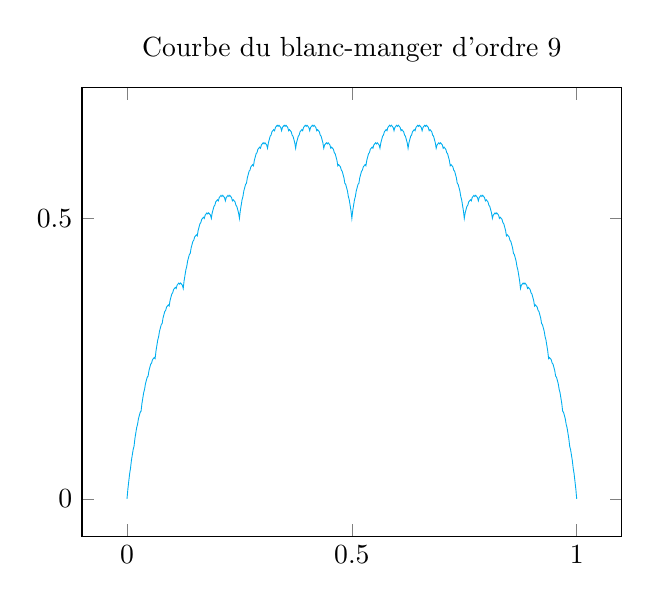
\begin{tikzpicture}

\begin{axis}[
title={Courbe du blanc-manger d'ordre 9},
xtick={0, 1/2, 1}, 
ytick={0, 1/2, 1}
]
\addplot [line width=0.32pt, cyan]
table {%
0 0
0.001953125 0.017578125
0.00390625 0.03125
0.005859375 0.044921875
0.0078125 0.0546875
0.009765625 0.068359375
0.01171875 0.078125
0.013671875 0.087890625
0.015625 0.09375
0.017578125 0.107421875
0.01953125 0.1171875
0.021484375 0.126953125
0.0234375 0.1328125
0.025390625 0.142578125
0.02734375 0.1484375
0.029296875 0.154296875
0.03125 0.15625
0.033203125 0.169921875
0.03515625 0.1796875
0.037109375 0.189453125
0.0390625 0.1953125
0.041015625 0.205078125
0.04296875 0.2109375
0.044921875 0.216796875
0.046875 0.21875
0.048828125 0.228515625
0.05078125 0.234375
0.052734375 0.240234375
0.0546875 0.2421875
0.056640625 0.248046875
0.05859375 0.25
0.060546875 0.251953125
0.0625 0.25
0.064453125 0.263671875
0.06640625 0.2734375
0.068359375 0.283203125
0.0703125 0.2890625
0.072265625 0.298828125
0.07421875 0.3046875
0.076171875 0.310546875
0.078125 0.3125
0.080078125 0.322265625
0.08203125 0.328125
0.083984375 0.333984375
0.0859375 0.3359375
0.087890625 0.341796875
0.08984375 0.34375
0.091796875 0.345703125
0.09375 0.34375
0.095703125 0.353515625
0.09765625 0.359375
0.099609375 0.365234375
0.1015625 0.3671875
0.103515625 0.373046875
0.10546875 0.375
0.107421875 0.376953125
0.109375 0.375
0.111328125 0.380859375
0.11328125 0.3828125
0.115234375 0.384765625
0.1171875 0.3828125
0.119140625 0.384765625
0.12109375 0.3828125
0.123046875 0.380859375
0.125 0.375
0.126953125 0.388671875
0.12890625 0.3984375
0.130859375 0.408203125
0.1328125 0.4140625
0.134765625 0.423828125
0.13671875 0.4296875
0.138671875 0.435546875
0.140625 0.4375
0.142578125 0.447265625
0.14453125 0.453125
0.146484375 0.458984375
0.1484375 0.4609375
0.150390625 0.466796875
0.15234375 0.46875
0.154296875 0.470703125
0.15625 0.46875
0.158203125 0.478515625
0.16015625 0.484375
0.162109375 0.490234375
0.1640625 0.4921875
0.166015625 0.498046875
0.16796875 0.5
0.169921875 0.501953125
0.171875 0.5
0.173828125 0.505859375
0.17578125 0.5078125
0.177734375 0.509765625
0.1796875 0.5078125
0.181640625 0.509765625
0.18359375 0.5078125
0.185546875 0.505859375
0.1875 0.5
0.189453125 0.509765625
0.19140625 0.515625
0.193359375 0.521484375
0.1953125 0.5234375
0.197265625 0.529296875
0.19921875 0.53125
0.201171875 0.533203125
0.203125 0.53125
0.205078125 0.537109375
0.20703125 0.5390625
0.208984375 0.541015625
0.2109375 0.5390625
0.212890625 0.541015625
0.21484375 0.5390625
0.216796875 0.537109375
0.21875 0.53125
0.220703125 0.537109375
0.22265625 0.5390625
0.224609375 0.541015625
0.2265625 0.5390625
0.228515625 0.541015625
0.23046875 0.5390625
0.232421875 0.537109375
0.234375 0.53125
0.236328125 0.533203125
0.23828125 0.53125
0.240234375 0.529296875
0.2421875 0.5234375
0.244140625 0.521484375
0.24609375 0.515625
0.248046875 0.509765625
0.25 0.5
0.251953125 0.513671875
0.25390625 0.5234375
0.255859375 0.533203125
0.2578125 0.5390625
0.259765625 0.548828125
0.26171875 0.5546875
0.263671875 0.560546875
0.265625 0.5625
0.267578125 0.572265625
0.26953125 0.578125
0.271484375 0.583984375
0.2734375 0.5859375
0.275390625 0.591796875
0.27734375 0.59375
0.279296875 0.595703125
0.28125 0.59375
0.283203125 0.603515625
0.28515625 0.609375
0.287109375 0.615234375
0.2890625 0.6171875
0.291015625 0.623046875
0.29296875 0.625
0.294921875 0.626953125
0.296875 0.625
0.298828125 0.630859375
0.30078125 0.6328125
0.302734375 0.634765625
0.3046875 0.6328125
0.306640625 0.634765625
0.30859375 0.6328125
0.310546875 0.630859375
0.3125 0.625
0.314453125 0.634765625
0.31640625 0.640625
0.318359375 0.646484375
0.3203125 0.6484375
0.322265625 0.654296875
0.32421875 0.65625
0.326171875 0.658203125
0.328125 0.65625
0.330078125 0.662109375
0.33203125 0.6640625
0.333984375 0.666015625
0.3359375 0.6640625
0.337890625 0.666015625
0.33984375 0.6640625
0.341796875 0.662109375
0.34375 0.65625
0.345703125 0.662109375
0.34765625 0.6640625
0.349609375 0.666015625
0.3515625 0.6640625
0.353515625 0.666015625
0.35546875 0.6640625
0.357421875 0.662109375
0.359375 0.65625
0.361328125 0.658203125
0.36328125 0.65625
0.365234375 0.654296875
0.3671875 0.6484375
0.369140625 0.646484375
0.37109375 0.640625
0.373046875 0.634765625
0.375 0.625
0.376953125 0.634765625
0.37890625 0.640625
0.380859375 0.646484375
0.3828125 0.6484375
0.384765625 0.654296875
0.38671875 0.65625
0.388671875 0.658203125
0.390625 0.65625
0.392578125 0.662109375
0.39453125 0.6640625
0.396484375 0.666015625
0.3984375 0.6640625
0.400390625 0.666015625
0.40234375 0.6640625
0.404296875 0.662109375
0.40625 0.65625
0.408203125 0.662109375
0.41015625 0.6640625
0.412109375 0.666015625
0.4140625 0.6640625
0.416015625 0.666015625
0.41796875 0.6640625
0.419921875 0.662109375
0.421875 0.65625
0.423828125 0.658203125
0.42578125 0.65625
0.427734375 0.654296875
0.4296875 0.6484375
0.431640625 0.646484375
0.43359375 0.640625
0.435546875 0.634765625
0.4375 0.625
0.439453125 0.630859375
0.44140625 0.6328125
0.443359375 0.634765625
0.4453125 0.6328125
0.447265625 0.634765625
0.44921875 0.6328125
0.451171875 0.630859375
0.453125 0.625
0.455078125 0.626953125
0.45703125 0.625
0.458984375 0.623046875
0.4609375 0.6171875
0.462890625 0.615234375
0.46484375 0.609375
0.466796875 0.603515625
0.46875 0.59375
0.470703125 0.595703125
0.47265625 0.59375
0.474609375 0.591796875
0.4765625 0.5859375
0.478515625 0.583984375
0.48046875 0.578125
0.482421875 0.572265625
0.484375 0.5625
0.486328125 0.560546875
0.48828125 0.5546875
0.490234375 0.548828125
0.4921875 0.5390625
0.494140625 0.533203125
0.49609375 0.5234375
0.498046875 0.513671875
0.5 0.5
0.501953125 0.513671875
0.50390625 0.5234375
0.505859375 0.533203125
0.5078125 0.5390625
0.509765625 0.548828125
0.51171875 0.5546875
0.513671875 0.560546875
0.515625 0.5625
0.517578125 0.572265625
0.51953125 0.578125
0.521484375 0.583984375
0.5234375 0.5859375
0.525390625 0.591796875
0.52734375 0.59375
0.529296875 0.595703125
0.53125 0.59375
0.533203125 0.603515625
0.53515625 0.609375
0.537109375 0.615234375
0.5390625 0.6171875
0.541015625 0.623046875
0.54296875 0.625
0.544921875 0.626953125
0.546875 0.625
0.548828125 0.630859375
0.55078125 0.6328125
0.552734375 0.634765625
0.5546875 0.6328125
0.556640625 0.634765625
0.55859375 0.6328125
0.560546875 0.630859375
0.5625 0.625
0.564453125 0.634765625
0.56640625 0.640625
0.568359375 0.646484375
0.5703125 0.6484375
0.572265625 0.654296875
0.57421875 0.65625
0.576171875 0.658203125
0.578125 0.65625
0.580078125 0.662109375
0.58203125 0.6640625
0.583984375 0.666015625
0.5859375 0.6640625
0.587890625 0.666015625
0.58984375 0.6640625
0.591796875 0.662109375
0.59375 0.65625
0.595703125 0.662109375
0.59765625 0.6640625
0.599609375 0.666015625
0.6015625 0.6640625
0.603515625 0.666015625
0.60546875 0.6640625
0.607421875 0.662109375
0.609375 0.65625
0.611328125 0.658203125
0.61328125 0.65625
0.615234375 0.654296875
0.6171875 0.6484375
0.619140625 0.646484375
0.62109375 0.640625
0.623046875 0.634765625
0.625 0.625
0.626953125 0.634765625
0.62890625 0.640625
0.630859375 0.646484375
0.6328125 0.6484375
0.634765625 0.654296875
0.63671875 0.65625
0.638671875 0.658203125
0.640625 0.65625
0.642578125 0.662109375
0.64453125 0.6640625
0.646484375 0.666015625
0.6484375 0.6640625
0.650390625 0.666015625
0.65234375 0.6640625
0.654296875 0.662109375
0.65625 0.65625
0.658203125 0.662109375
0.66015625 0.6640625
0.662109375 0.666015625
0.6640625 0.6640625
0.666015625 0.666015625
0.66796875 0.6640625
0.669921875 0.662109375
0.671875 0.65625
0.673828125 0.658203125
0.67578125 0.65625
0.677734375 0.654296875
0.6796875 0.6484375
0.681640625 0.646484375
0.68359375 0.640625
0.685546875 0.634765625
0.6875 0.625
0.689453125 0.630859375
0.69140625 0.6328125
0.693359375 0.634765625
0.6953125 0.6328125
0.697265625 0.634765625
0.69921875 0.6328125
0.701171875 0.630859375
0.703125 0.625
0.705078125 0.626953125
0.70703125 0.625
0.708984375 0.623046875
0.7109375 0.6171875
0.712890625 0.615234375
0.71484375 0.609375
0.716796875 0.603515625
0.71875 0.59375
0.720703125 0.595703125
0.72265625 0.59375
0.724609375 0.591796875
0.7265625 0.5859375
0.728515625 0.583984375
0.73046875 0.578125
0.732421875 0.572265625
0.734375 0.5625
0.736328125 0.560546875
0.73828125 0.5546875
0.740234375 0.548828125
0.7421875 0.5390625
0.744140625 0.533203125
0.74609375 0.5234375
0.748046875 0.513671875
0.75 0.5
0.751953125 0.509765625
0.75390625 0.515625
0.755859375 0.521484375
0.7578125 0.5234375
0.759765625 0.529296875
0.76171875 0.53125
0.763671875 0.533203125
0.765625 0.53125
0.767578125 0.537109375
0.76953125 0.5390625
0.771484375 0.541015625
0.7734375 0.5390625
0.775390625 0.541015625
0.77734375 0.5390625
0.779296875 0.537109375
0.78125 0.53125
0.783203125 0.537109375
0.78515625 0.5390625
0.787109375 0.541015625
0.7890625 0.5390625
0.791015625 0.541015625
0.79296875 0.5390625
0.794921875 0.537109375
0.796875 0.53125
0.798828125 0.533203125
0.80078125 0.53125
0.802734375 0.529296875
0.8046875 0.5234375
0.806640625 0.521484375
0.80859375 0.515625
0.810546875 0.509765625
0.8125 0.5
0.814453125 0.505859375
0.81640625 0.5078125
0.818359375 0.509765625
0.8203125 0.5078125
0.822265625 0.509765625
0.82421875 0.5078125
0.826171875 0.505859375
0.828125 0.5
0.830078125 0.501953125
0.83203125 0.5
0.833984375 0.498046875
0.8359375 0.4921875
0.837890625 0.490234375
0.83984375 0.484375
0.841796875 0.478515625
0.84375 0.46875
0.845703125 0.470703125
0.84765625 0.46875
0.849609375 0.466796875
0.8515625 0.4609375
0.853515625 0.458984375
0.85546875 0.453125
0.857421875 0.447265625
0.859375 0.4375
0.861328125 0.435546875
0.86328125 0.4296875
0.865234375 0.423828125
0.8671875 0.4140625
0.869140625 0.408203125
0.87109375 0.3984375
0.873046875 0.388671875
0.875 0.375
0.876953125 0.380859375
0.87890625 0.3828125
0.880859375 0.384765625
0.8828125 0.3828125
0.884765625 0.384765625
0.88671875 0.3828125
0.888671875 0.380859375
0.890625 0.375
0.892578125 0.376953125
0.89453125 0.375
0.896484375 0.373046875
0.8984375 0.3671875
0.900390625 0.365234375
0.90234375 0.359375
0.904296875 0.353515625
0.90625 0.34375
0.908203125 0.345703125
0.91015625 0.34375
0.912109375 0.341796875
0.9140625 0.3359375
0.916015625 0.333984375
0.91796875 0.328125
0.919921875 0.322265625
0.921875 0.3125
0.923828125 0.310546875
0.92578125 0.3046875
0.927734375 0.298828125
0.9296875 0.2890625
0.931640625 0.283203125
0.93359375 0.2734375
0.935546875 0.263671875
0.9375 0.25
0.939453125 0.251953125
0.94140625 0.25
0.943359375 0.248046875
0.9453125 0.2421875
0.947265625 0.240234375
0.94921875 0.234375
0.951171875 0.228515625
0.953125 0.21875
0.955078125 0.216796875
0.95703125 0.2109375
0.958984375 0.205078125
0.9609375 0.1953125
0.962890625 0.189453125
0.96484375 0.1796875
0.966796875 0.169921875
0.96875 0.15625
0.970703125 0.154296875
0.97265625 0.1484375
0.974609375 0.142578125
0.9765625 0.1328125
0.978515625 0.126953125
0.98046875 0.1171875
0.982421875 0.107421875
0.984375 0.09375
0.986328125 0.087890625
0.98828125 0.078125
0.990234375 0.068359375
0.9921875 0.0546875
0.994140625 0.044921875
0.99609375 0.03125
0.998046875 0.017578125
1 0
};
\end{axis}

\end{tikzpicture}

\end{figure}

\begin{defi}{Distance à $\Z$}
    Pour tout $x \in \R$, on définit la fonction $\ll x \gg$ distance de $x$ à $\Z$. 
\end{defi}

\begin{prop}{Expression de $\ll \cdot \gg$}
$$\ll \cdot \gg : x \mapsto \left| x - \left\lfloor x + \frac{1}{2} \right\rfloor \right|$$
\end{prop}

\begin{preuve}
    
\end{preuve}

\begin{defi}{Courbe du blancmanger ou de \textsc{Takagi}}
On définit cette courbe par la fonction
    \begin{alignat*}{2}
        \tau\ :\ [0,1]\ &\longrightarrow\ [0,1]\\
        x\ &\longmapsto\ \sum\limits_{k=0}^\infty \frac{1}{2^k} \ll 2^k x \gg.
    \end{alignat*}
\end{defi}

\subsection{Courbe de \textsc{Bolzano}-\textsc{Lebesgue}}    

\begin{defi}{Courbe de \textsc{Bolzano}-\textsc{Lebesgue}}
    On pose $I \defeq [0, 1]$ et $(f_n)$ la suite de fonctions définie par
    \begin{itemize}
        \item $f_0(x) = x.$
        \item $f_n$ est affine sur $\left[ \frac{k}{3^n}, \frac{k+1}{3^n} \right]$ pour tout $k \in \llbracket 0, 3^n - 1 \rrbracket$.
        \item $f_n$ et $f_{n-1}$ sont égales en $\frac{3k}{3^n}$, $\frac{3k+1}{3^n}$ et $\frac{3k+2}{3^n}$ pour tout $k \in \llbracket 0, 3^n-1 \rrbracket$.
    \end{itemize}
\end{defi}

\subsection{Densité de $F$ dans $E$}

\begin{theo}{}
    $F$ est dense dans $E$ pour la topologie uniforme.
\end{theo}

\begin{preuve}
    \marginnote[0cm]{\url{https://share.miple.co/content/XEZ7y9BayeSN1}}
    Soient $f \in E$ et $W \in F$. La fonction $f - W$ est continue sur $[0, 1]$ donc peut être approchée uniformément par une suite $(A_n)_{n \in \N}$ de fonctions polynomiales définies sur $[0, 1]$ d'après le théorème de \textsc{Weierstrass}. \\
    Pour tout $n \in \N$, notons $B_n \defeq A_n + W$. La fonction $B_n$ est continue et nulle part dérivable puisque si $(B_n)_{n \in \N}$ était dérivable en $x \in [0, 1]$, la fonction $W$ le serait aussi. La suite $(B_n)_{n \in \N}$ est donc une suite de fonctions continues sur $[0,1]$ et nulle part dérivable qui converge uniformément vers la fonction $f$.
\end{preuve}

- \url{http://christophebertault.fr/documents/articles/Article - Une famille nombreuse de fonctions continues partout derivables nulle part.pdf} \\
- lire le paragraphe éponyme dans \cite{contre-exemples} page 350. \\

\section{A rajouter}

\begin{itemize}
    \item Intégrale à paramètre vs. série de fonctions
    \item Développements asymptotiques de sommes de séries de fonctions
\end{itemize}